\documentclass[11pt,a4paper]{article}
\usepackage[utf8]{inputenc}
\usepackage[T1]{fontenc}
\usepackage[french]{babel}
\usepackage{graphicx}
\usepackage{geometry}
\geometry{a4paper, margin=2cm}
\usepackage{hyperref}
\usepackage{float}

\begin{document}

\begin{titlepage}
    \centering
    \vspace*{2cm}
    
    {\scshape\LARGE Université de Montpellier \par}
    \vspace{1.5cm}
    {\scshape\Large Master 1 - Programmation Mobile\par}
    \vspace{2cm}
    
    \rule{\linewidth}{0.5mm} \\[0.6cm]
    {\Huge\bfseries Projet : Application Traveling\par}
    \vspace{0.5cm}
    {\Large\itshape Rendu Semaine 1 : Analyse Fonctionnelle et Maquettes\par}
    \rule{\linewidth}{0.5mm} \\[2cm]
    
    \vspace{1.5cm}
    
    {\Large\bfseries Présenté par :}\\[0.8cm]
    {\LARGE AMMARI Reda \\ ALJIBBAOUI Tala \par}
    
    \vfill
    
    {\large \today\par}
\end{titlepage}

\newpage


\section{Analyse Fonctionnelle : Diagramme de Cas d'Utilisation}
Le diagramme de cas d'utilisation ci-dessous présente la structure globale de l'application "Traveling", divisée en deux modules interactifs : TravelShare (partage de contenu) et TravelPath (génération de parcours personnalisés). Les interactions avec les API externes (Météo, Réservation) sont également modélisées.

\begin{figure}[H]
    \centering
    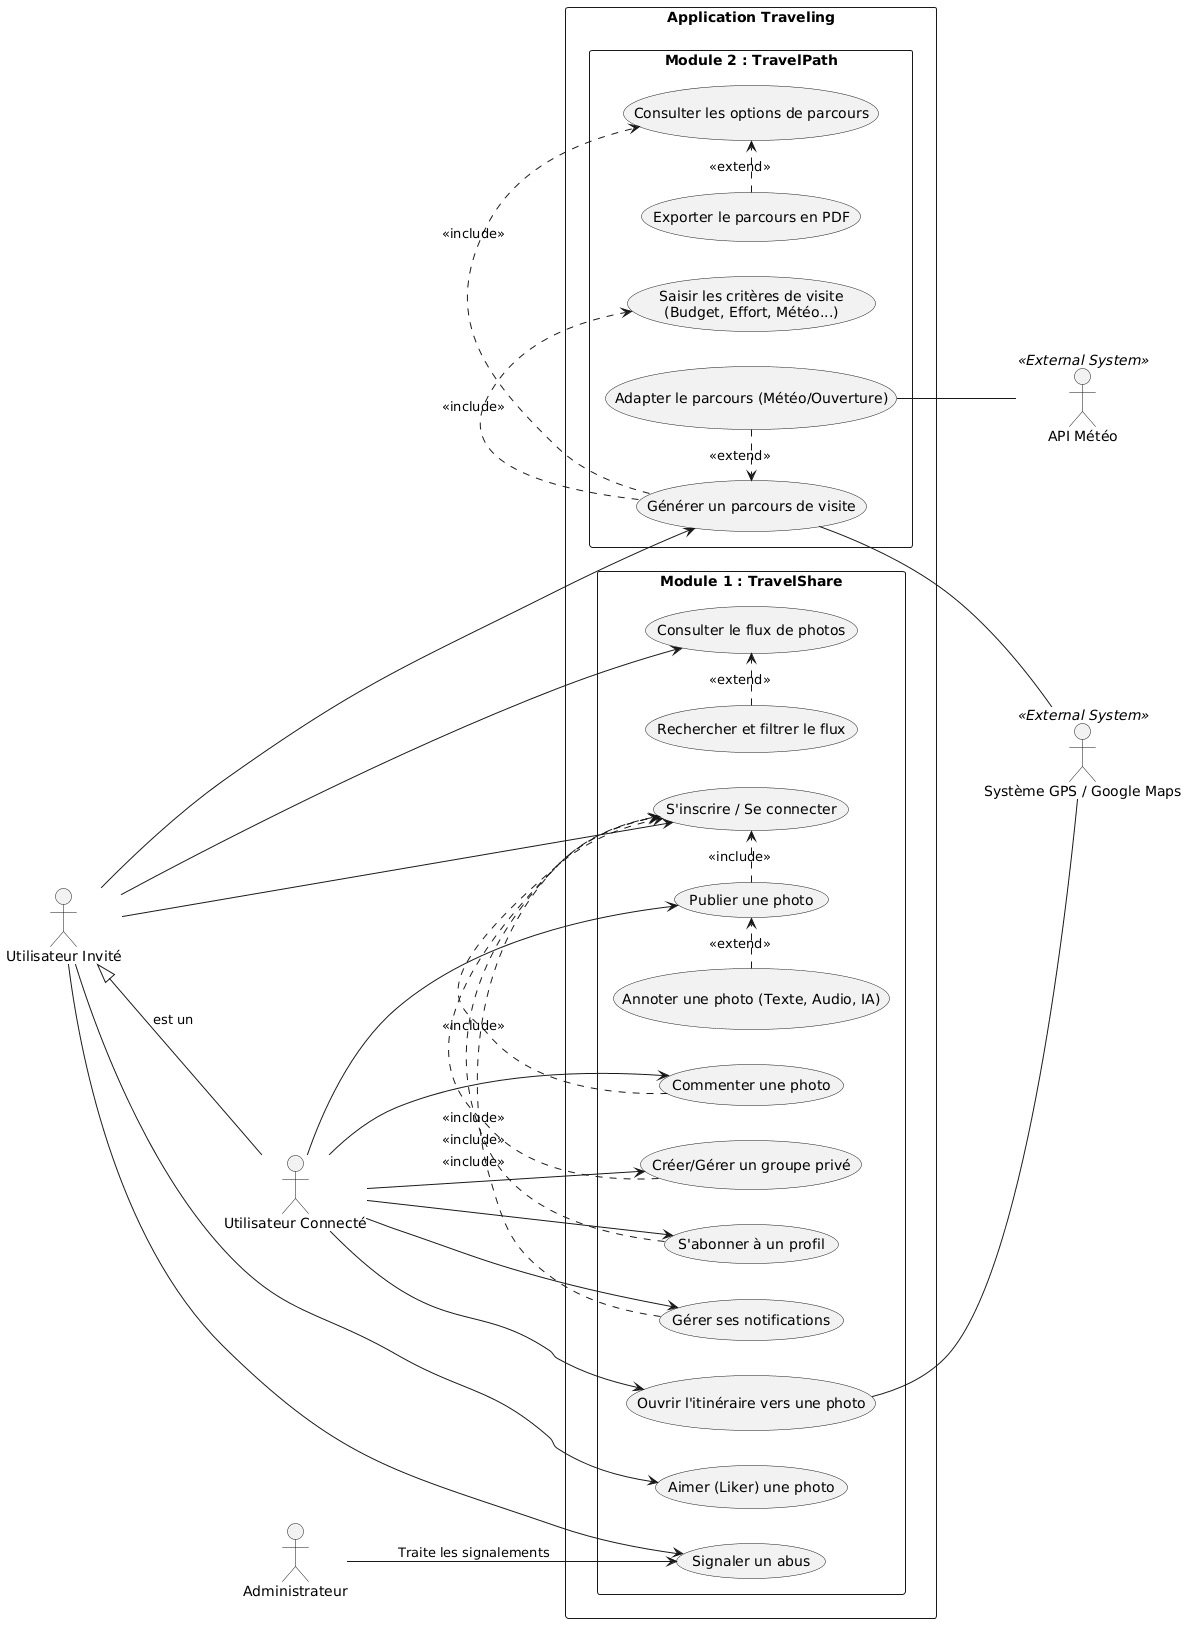
\includegraphics[width=\textwidth,height=0.8\textheight,keepaspectratio]{uml.jpg}
    \caption{Diagramme de cas d'utilisation global (TravelShare et TravelPath)}
\end{figure}

\newpage
\section{Maquettes de l'Application (Figma)}
Cette section présente les écrans principaux de l'application conçus sous Figma, permettant de visualiser l'expérience utilisateur (UX/UI) pour la passerelle commune ainsi que pour les modules spécifiques. Le design est prévu avec des composants Material Design pour garantir une implémentation fluide du code Android en Java.

\subsection{Écran d'Accueil (La Passerelle)}
L'écran principal de l'application, agissant comme point d'entrée unique laissant le choix à l'utilisateur entre la partie réseau social/découverte et la partie planificateur de visite.

\begin{figure}[H]
    \centering
    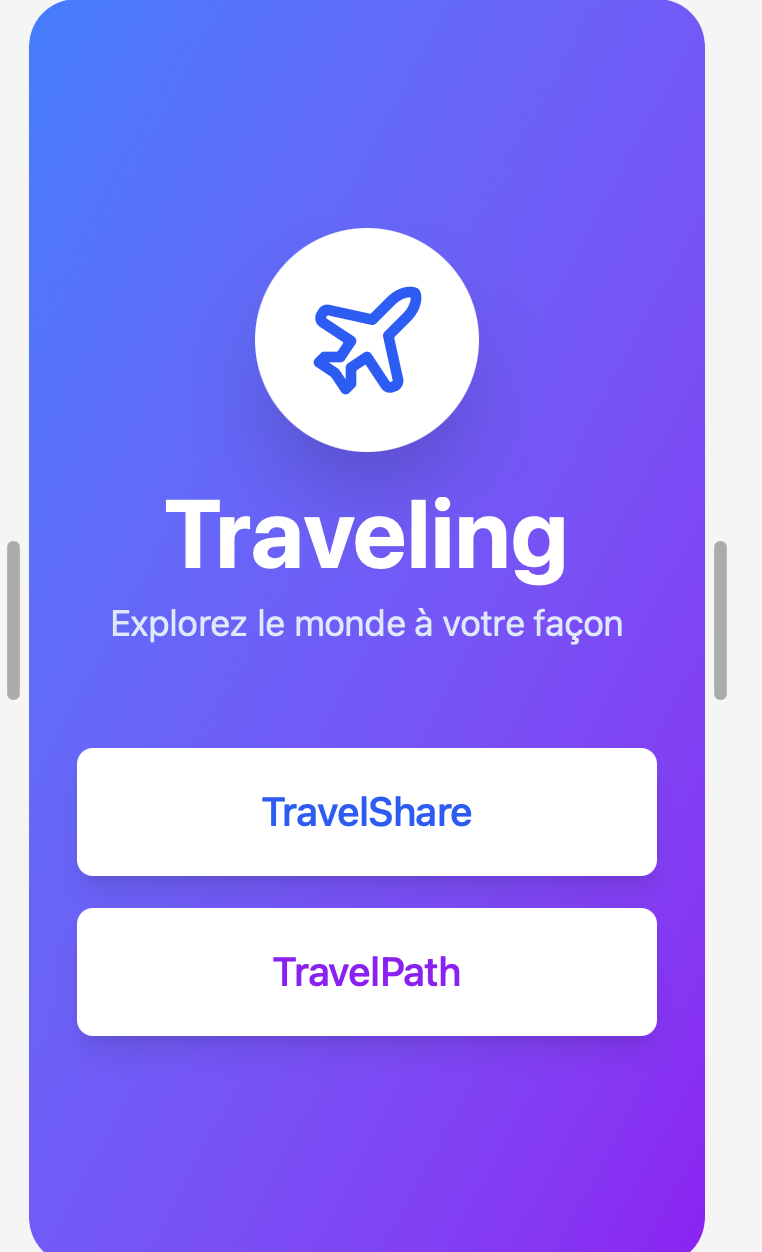
\includegraphics[width=0.6\textwidth]{home.png}
    \caption{Écran d'Accueil - Accès aux services TravelShare et TravelPath}
\end{figure}

\newpage
\subsection{Module 1 : TravelShare}
Le flux de photos principal. On y retrouve l'auteur, le lieu, et les boutons d'interaction obligatoires (Like, Commentaire) selon les spécifications. Le bouton "Plus" a été ajouté pour permettre l'ajout de nouvelles photos.

\begin{figure}[H]
    \centering
    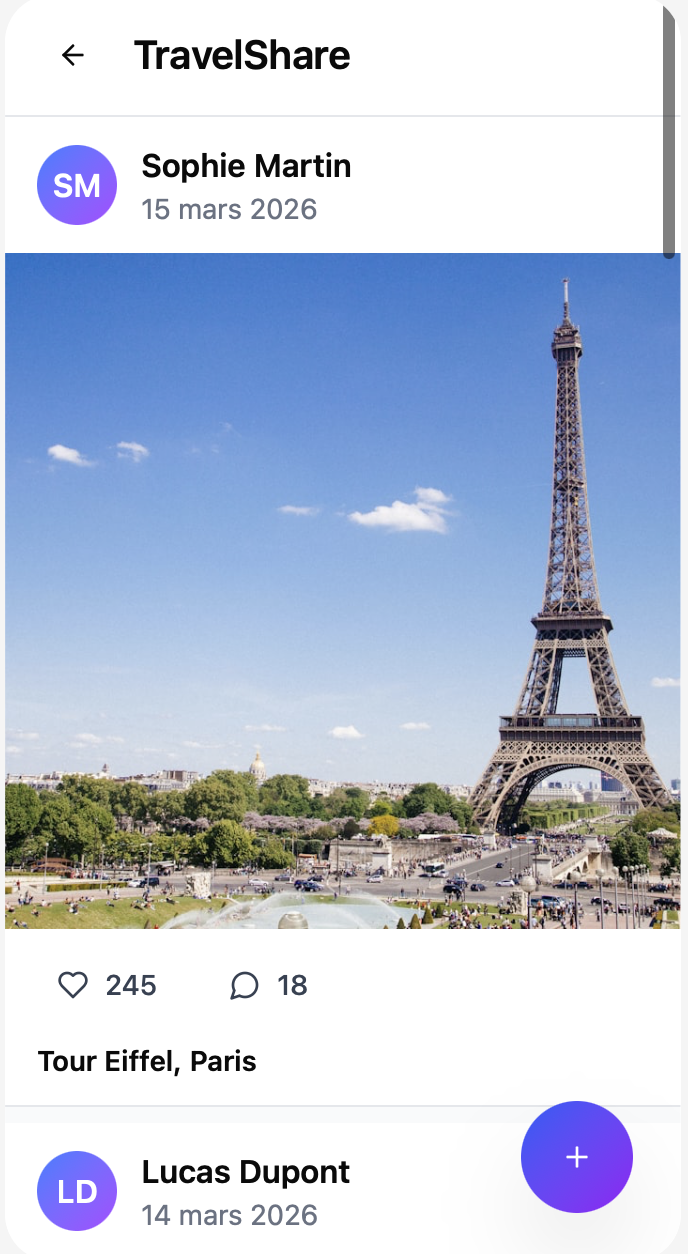
\includegraphics[width=0.7\textwidth]{travelshare.png}
    \caption{Le flux public de photos avec bouton de création (TravelShare)}
\end{figure}

\newpage
\subsection{Module 2 : TravelPath - Formulaire}
Formulaire permettant de renseigner les contraintes et critères pour la génération d'un parcours personnalisé (budget, destination, météo attendue).

\begin{figure}[H]
    \centering
    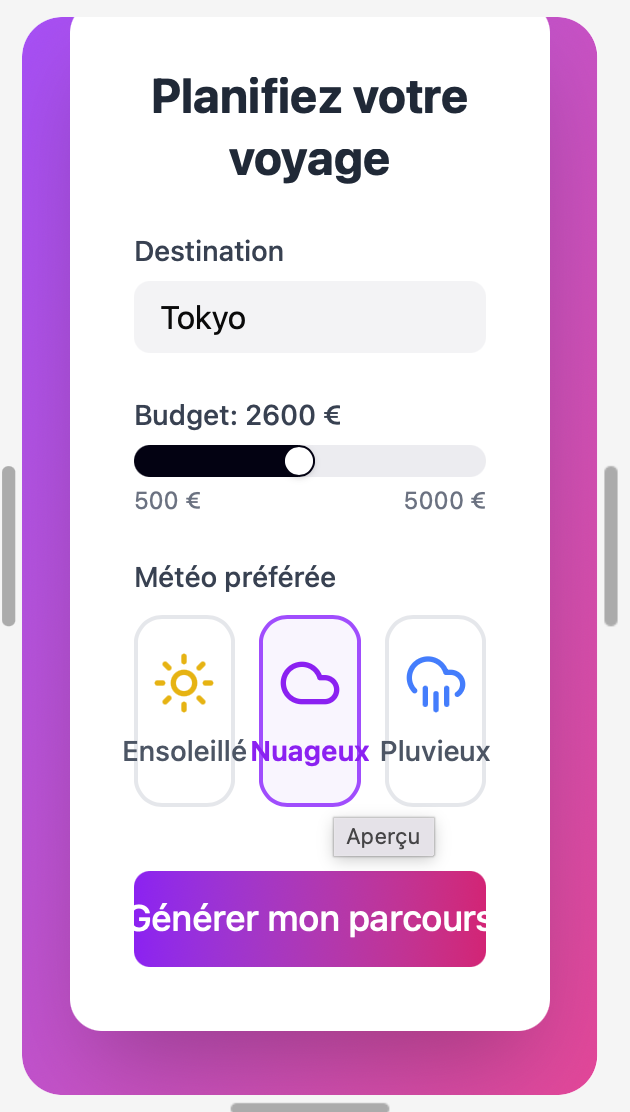
\includegraphics[width=0.7\textwidth]{travelpath_form.png}
    \caption{Saisie des critères de visite (TravelPath)}
\end{figure}

\newpage
\subsection{Module 2 : TravelPath - Résultat de l'Itinéraire}
Affichage schématisé montrant la chronologie logicielle du parcours généré (timeline), incluant la carte de prévisualisation de l'itinéraire et les options d'export.

\begin{figure}[H]
    \centering
    \begin{minipage}{0.48\textwidth}
        \centering
        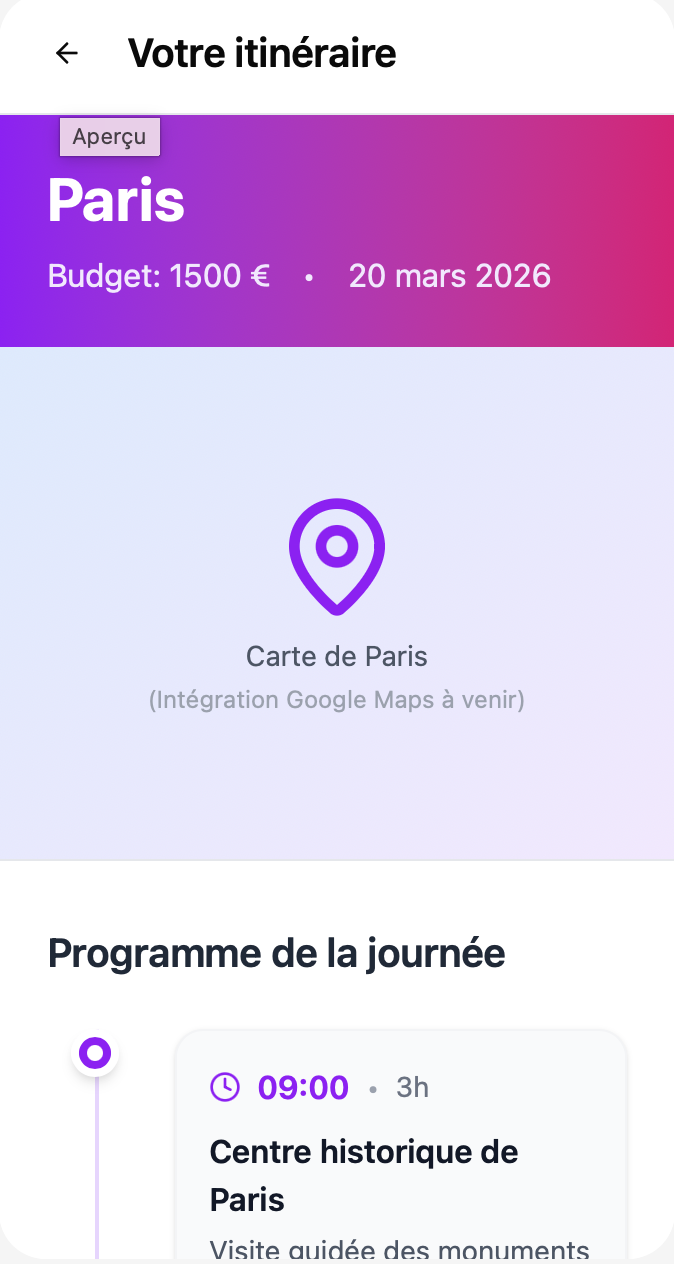
\includegraphics[width=\textwidth]{travelpath_result_map.png}
        \caption{Haut de l'écran (Carte et début du parcours)}
    \end{minipage}\hfill
    \begin{minipage}{0.48\textwidth}
        \centering
        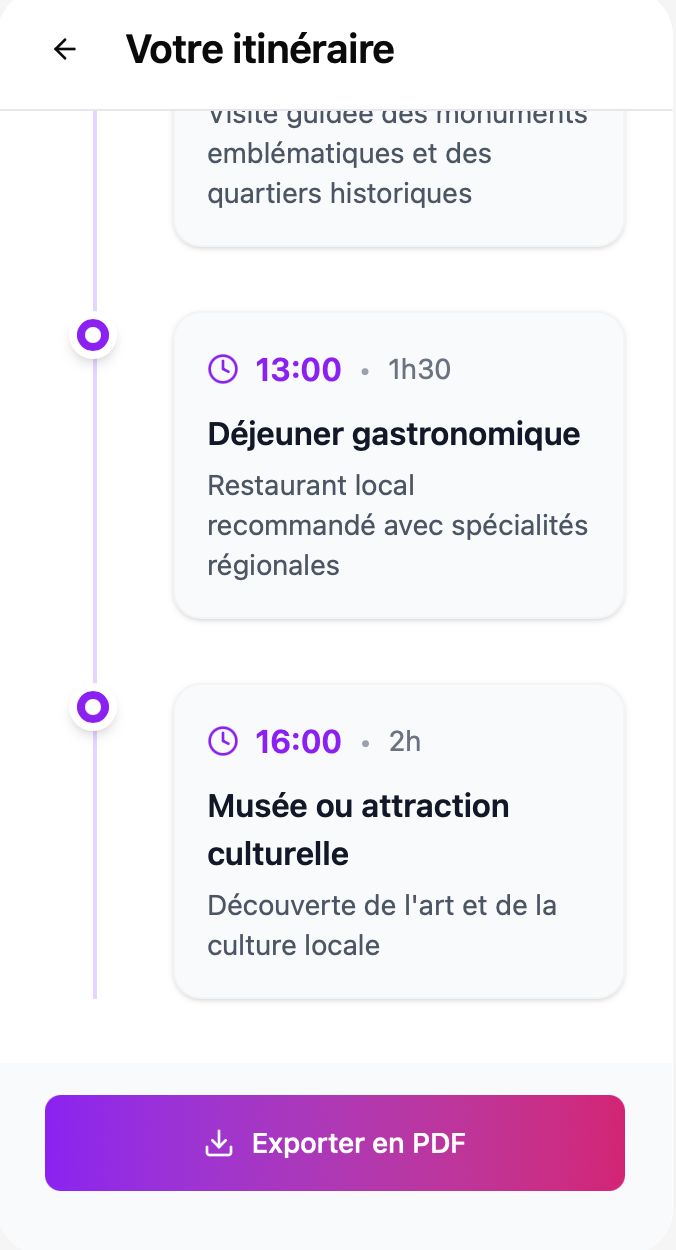
\includegraphics[width=\textwidth]{travelpath_result_pdf.png}
        \caption{Bas de l'écran (Suite du parcours et Export PDF)}
    \end{minipage}
\end{figure}

\end{document}
